\section{画像外の知識の改善の試み}
\label{sec_outside}
発話の型は6区分を信頼性の低いラベルとして扱うことにしたため，以降は画像外の知識の改善に絞った．
本章では，教師ラベルの改善，生徒の構成の変更，ボケの文の再出現の回数の3つの試みを述べる．

\subsection{教師の指示の改善}
教師ラベルの画像外の知識は，学習用の目視ラベル931件との一致が F1 0.59にとどまる．
そこで，32B の教師に画像外の知識だけを問う指示を3つ追加し，目視ラベルのある1,551件で比較した．
追加した指示は，先に元ネタ（作品・人物・台詞・歌詞・CM・流行語・ネットの定型などの引用・もじり・パロディ）を具体的に書かせてから種類・画像内か・必要かを問う指示（src），src に例を加えた指示（src\_fs），src を温度0.7で5回生成して多数決をとる指示（src\_sc）である．

表\ref{tab_outside_teacher}に結果を示す．
元ネタを書き出させると再現率は上がったが，固有名詞や言い回しをなんでも元ネタとみなして「はい」とするため適合率が大きく下がり，F1 はいずれも従来の指示（kt）を下回った．
32B の指示の変更では，教師ラベルを改善できなかった．

\begin{table}[t]
    \centering
    \caption{教師（32B）の画像外の知識の F1．括弧内は学習用931件での適合率と再現率．}
    \label{tab_outside_teacher}
    \small
    \setlength{\tabcolsep}{3pt}
    \begin{tabular}{@{}lccc@{}}
        \toprule
        指示 & 学習用931件 & dev & test \\
        \midrule
        kt（one\_kt\_cap） & \textbf{0.59}（0.54／0.65） & \textbf{0.58} & \textbf{0.67} \\
        src & 0.54（0.44／0.70） & 0.46 & 0.62 \\
        src\_fs & 0.54（0.44／0.68） & 0.55 & 0.64 \\
        src\_sc & 0.54（0.43／0.74） & 0.52 & 0.60 \\
        \bottomrule
    \end{tabular}
\end{table}

\subsection{生徒の構成の変更}
次の要素を変えて，二段階の学習を行った．
\begin{itemize}
    \item モデルの大きさ：InternVL3.5-8B と Qwen3-VL-8B．
    \item 損失の重み：(\ref{eq_loss})の $ \lambda $ を3とする．
    \item 疑似ラベル：段階2まで学習した Qwen3-VL-4B（最終評価用で0.69）で学習用のボケ34,634件の画像外の知識を付け直し，段階1の教師ラベルとする（自己学習\cite{ref_noisy_student}）．
    \item アンサンブル：複数のモデルの画像外の知識の確率の平均．
\end{itemize}
図\ref{fig_outside}と表\ref{tab_outside_student}に結果を示す．

\begin{figure}[t]
    \centering
    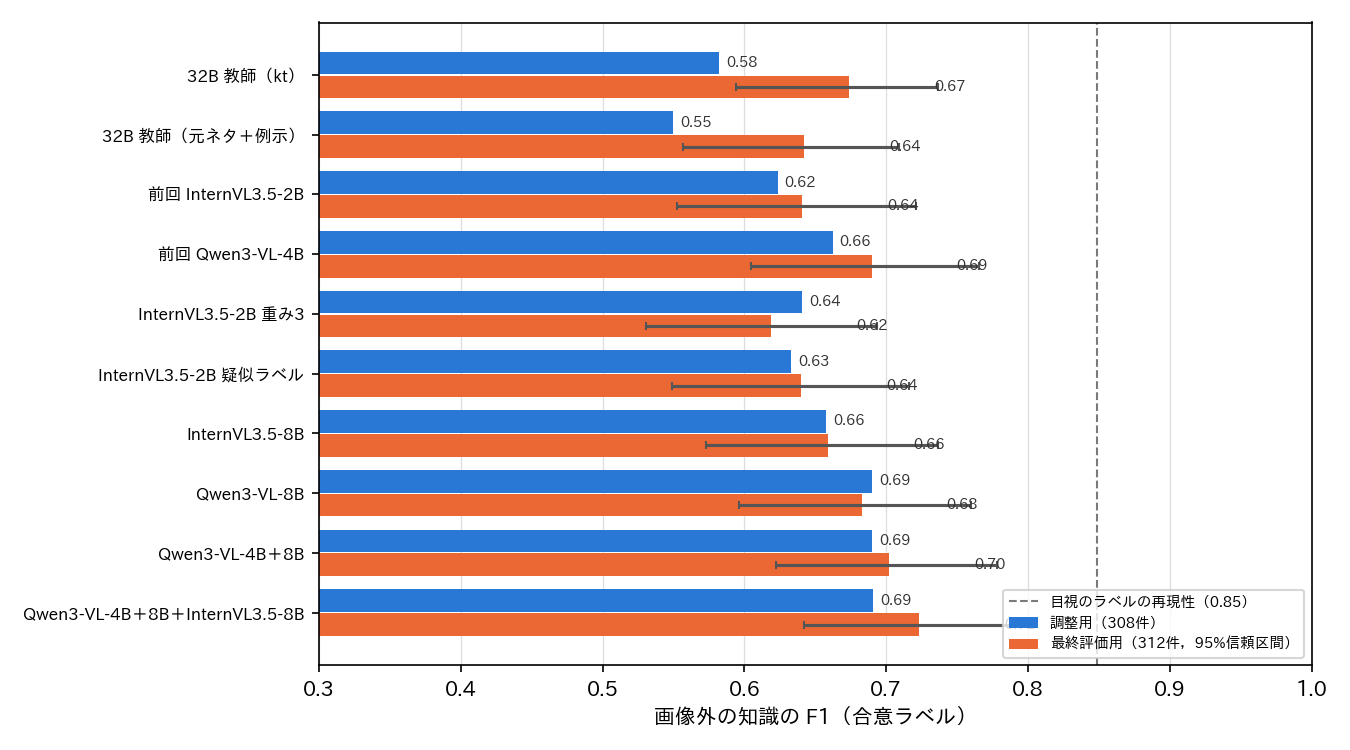
\includegraphics[width=\linewidth]{figures/fig_outside.png}
    \caption{画像外の知識の F1（合意ラベル）．最終評価用は95\%信頼区間を示す．破線は目視ラベルの再現性である．}
    \label{fig_outside}
\end{figure}

\begin{table}[t]
    \centering
    \caption{画像外の知識の改善の試み（段階1＋段階2．AUC は最終評価用）．}
    \label{tab_outside_student}
    \footnotesize
    \setlength{\tabcolsep}{3pt}
    \begin{tabular}{@{}lcccc@{}}
        \toprule
        方法 & dev & test & 95\%区間 & AUC \\
        \midrule
        Qwen3-VL-4B（$\lambda=1$） & 0.66 & 0.69 & 0.60--0.77 & 0.87 \\
        InternVL3.5-2B（$\lambda=1$） & 0.62 & 0.64 & 0.55--0.72 & 0.84 \\
        InternVL3.5-2B（$\lambda=3$） & 0.64 & 0.62 & 0.53--0.69 & 0.83 \\
        InternVL3.5-2B（$\lambda=3$，疑似） & 0.63 & 0.64 & 0.55--0.72 & 0.86 \\
        InternVL3.5-8B（$\lambda=3$） & 0.66 & 0.66 & 0.57--0.74 & 0.85 \\
        Qwen3-VL-8B（$\lambda=3$） & \textbf{0.69} & 0.68 & 0.60--0.76 & 0.85 \\
        Qwen3-VL-4B＋8B & \textbf{0.69} & \textbf{0.70} & 0.62--0.78 & 0.88 \\
        \bottomrule
    \end{tabular}
\end{table}

Qwen3-VL-8B は，調整用で 4B より0.03高かったが，最終評価用ではほぼ同じであった．
InternVL3.5 は 2B から 8B で0.02〜0.04上がったが，Qwen3-VL より低かった．
疑似ラベルは段階1の後では効果があり（最終評価用0.63から0.65），段階2の後では差がなくなった．
損失の重みは効果がなかった．
4B と 8B の確率の平均は，AUC と F1 をわずかに上げた．
いずれの改善も信頼区間の幅（約 $ \pm 0.08 $）より小さく，2〜8B のモデルと教師ラベルの組み合わせでは F1 0.66〜0.70で頭打ちになった．
なお，Qwen3-VL-8B の段階2の後の6区分は，調整用0.76，最終評価用0.74であった．

\subsection{ボケの文の再出現の回数}
有名な台詞や定型を引用するボケは，同じ文が多くのお題に繰り返し投稿されると考えた．
全てのボケの文を正規化（NFKC，小文字化，空白・記号の除去）し，同じ文が投稿されたお題の数を数え，自分のお題を除いた回数を特徴とした．
しかし，この回数の画像外の知識に対する AUC は0.53〜0.56にとどまった．
「なにこれ」「いらっしゃいませ」のような短く一般的な言葉も多くのお題に繰り返し投稿されるためであり，この特徴は用いなかった．

\subsection{誤りの分析}
Qwen3-VL-4B と 8B のアンサンブルの検証データ620件での誤りは，見逃し44件と誤検出51件であった．
表\ref{tab_errors}に例を示す．

\begin{table}[t]
    \centering
    \caption{画像外の知識の誤りの例（Qwen3-VL-4B＋8B）．括弧内は確率．}
    \label{tab_errors}
    \footnotesize
    \begin{tabular}{@{}p{0.16\linewidth}p{0.77\linewidth}@{}}
        \toprule
        種類 & ボケと元ネタ \\
        \midrule
        見逃し & 「バスケがしたいです。」（0.00，漫画の名台詞） \\
        & 「返事がない。ただの壁のようだ。」（0.02，ゲームの定型文のもじり） \\
        & 「俺か俺以外か」（0.00，タレントの決め台詞） \\
        & 「こうかはいまひとつのようだ」（0.10，ゲームの定型文） \\
        \midrule
        誤検出 & 「ジャムおじさんを基準にすると巨人の星」（1.00，画像は同じ作品） \\
        & 「くまモンに丸のみされたなっしー・・・。」（1.00） \\
        & 「だるまさんがこーろんだっ！」（0.99，一般の遊び） \\
        \bottomrule
    \end{tabular}
\end{table}

見逃しの大半は，有名な台詞・歌詞・ネットの定型の引用であった．
例えば，漫画の名台詞を借りた「バスケがしたいです。」，ゲームの定型文をもじった「返事がない。ただの壁のようだ。」，タレントの決め台詞である「俺か俺以外か」であり，字面は普通の日本語であるため，元ネタを知らないモデルには判定できない．
誤検出の多くは，画像に写っている作品の登場人物を画像外とするものであった．
例えば，アンパンマンの画像に対する「ジャムおじさん」や「バタコさん」を含むボケである．
また，固有名詞を含むだけで一般の知識で面白さが分かるボケも誤検出された．
見逃しは知識の量の問題であり，2〜8B のモデルの微調整では改善が限られる．
誤検出は画像に写っている作品の同定の問題であり，お題画像ごとに写っている作品を同定して入力に加えることで改善できる可能性がある．
